\documentclass[aspectratio=169]{beamer}

\usepackage{color}
\definecolor{airforceblue}{rgb}{0.36, 0.54, 0.66}
\definecolor{blue-green}{rgb}{0.0, 0.87, 0.87}
\definecolor{blue-violet}{rgb}{0.54, 0.17, 0.89}
\definecolor{cadet}{rgb}{0.33, 0.41, 0.47}
\definecolor{cordovan}{rgb}{0.54, 0.25, 0.27}

\mode<presentation>
{
    \usetheme{Madrid}
    \usefonttheme{professionalfonts} 
	\setbeamercolor{local structure}{fg=blue-green}
    \setbeamertemplate{itemize subitem}{\color{cordovan}$\blacktriangleright$}
}


\usepackage[utf8]{inputenc}
\usetheme{Madrid}
\usecolortheme{beaver}

\title{Comunicação em Datacenters}
\subtitle{Gerência de Redes}
\author[Leandro Silva, Luís Felipe] % (optional, for multiple authors)
{Leandro Souza da  Silva \\ Luís Felipe Mattos}
\institute{IC - Unicamp}


\date{ 06 de Dezembro de 2016 }
\logo{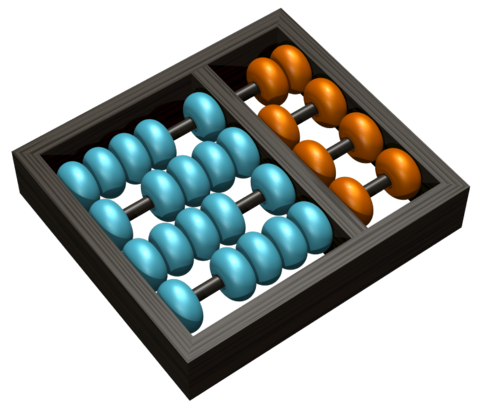
\includegraphics[height=1.0cm]{logo.png}}
 
\AtBeginSection[]
{
  \begin{frame}<beamer>{Sumário}
    \tableofcontents[currentsection, currentsubsection]
  \end{frame}
}

\AtBeginSubsection[]
{
  \begin{frame}<beamer>{Sumário}
    \tableofcontents[currentsection, currentsubsection]
  \end{frame}
}


\begin{document}

\frame{\titlepage}

\section{Introdução}
	\begin{frame} {Introdução}
	
		
	 \begin{itemize}
	 \setlength\itemsep{2em}
	 	\Large
	 	\item
	 		Com o crescimento da computação em nuvem, os datacenters passaram a receber funções novas.
	 		
	 \item
	  	Certas aplicações necessitam de certos requisitos:
	  	\begin{itemize}
	 		\item
	 			Escalabilidade
	 	
			\item
			 	Tolerância a Falhas
			\item
			 	Latêcia
			 	
			 \item
			 	Capacidade da Rede
			 \item
			 	Virtualização	 			
	 	\end{itemize}
	 		 	
	 \end{itemize}
		
	\end{frame}



\section{Motivação} 

	\begin{frame} {Motivação}
			
			\centering
			\Large
				 O consumo de dados pelos usuários está crescendo exponencialmente a cada ano.
				\begin{figure}[ht]    
				    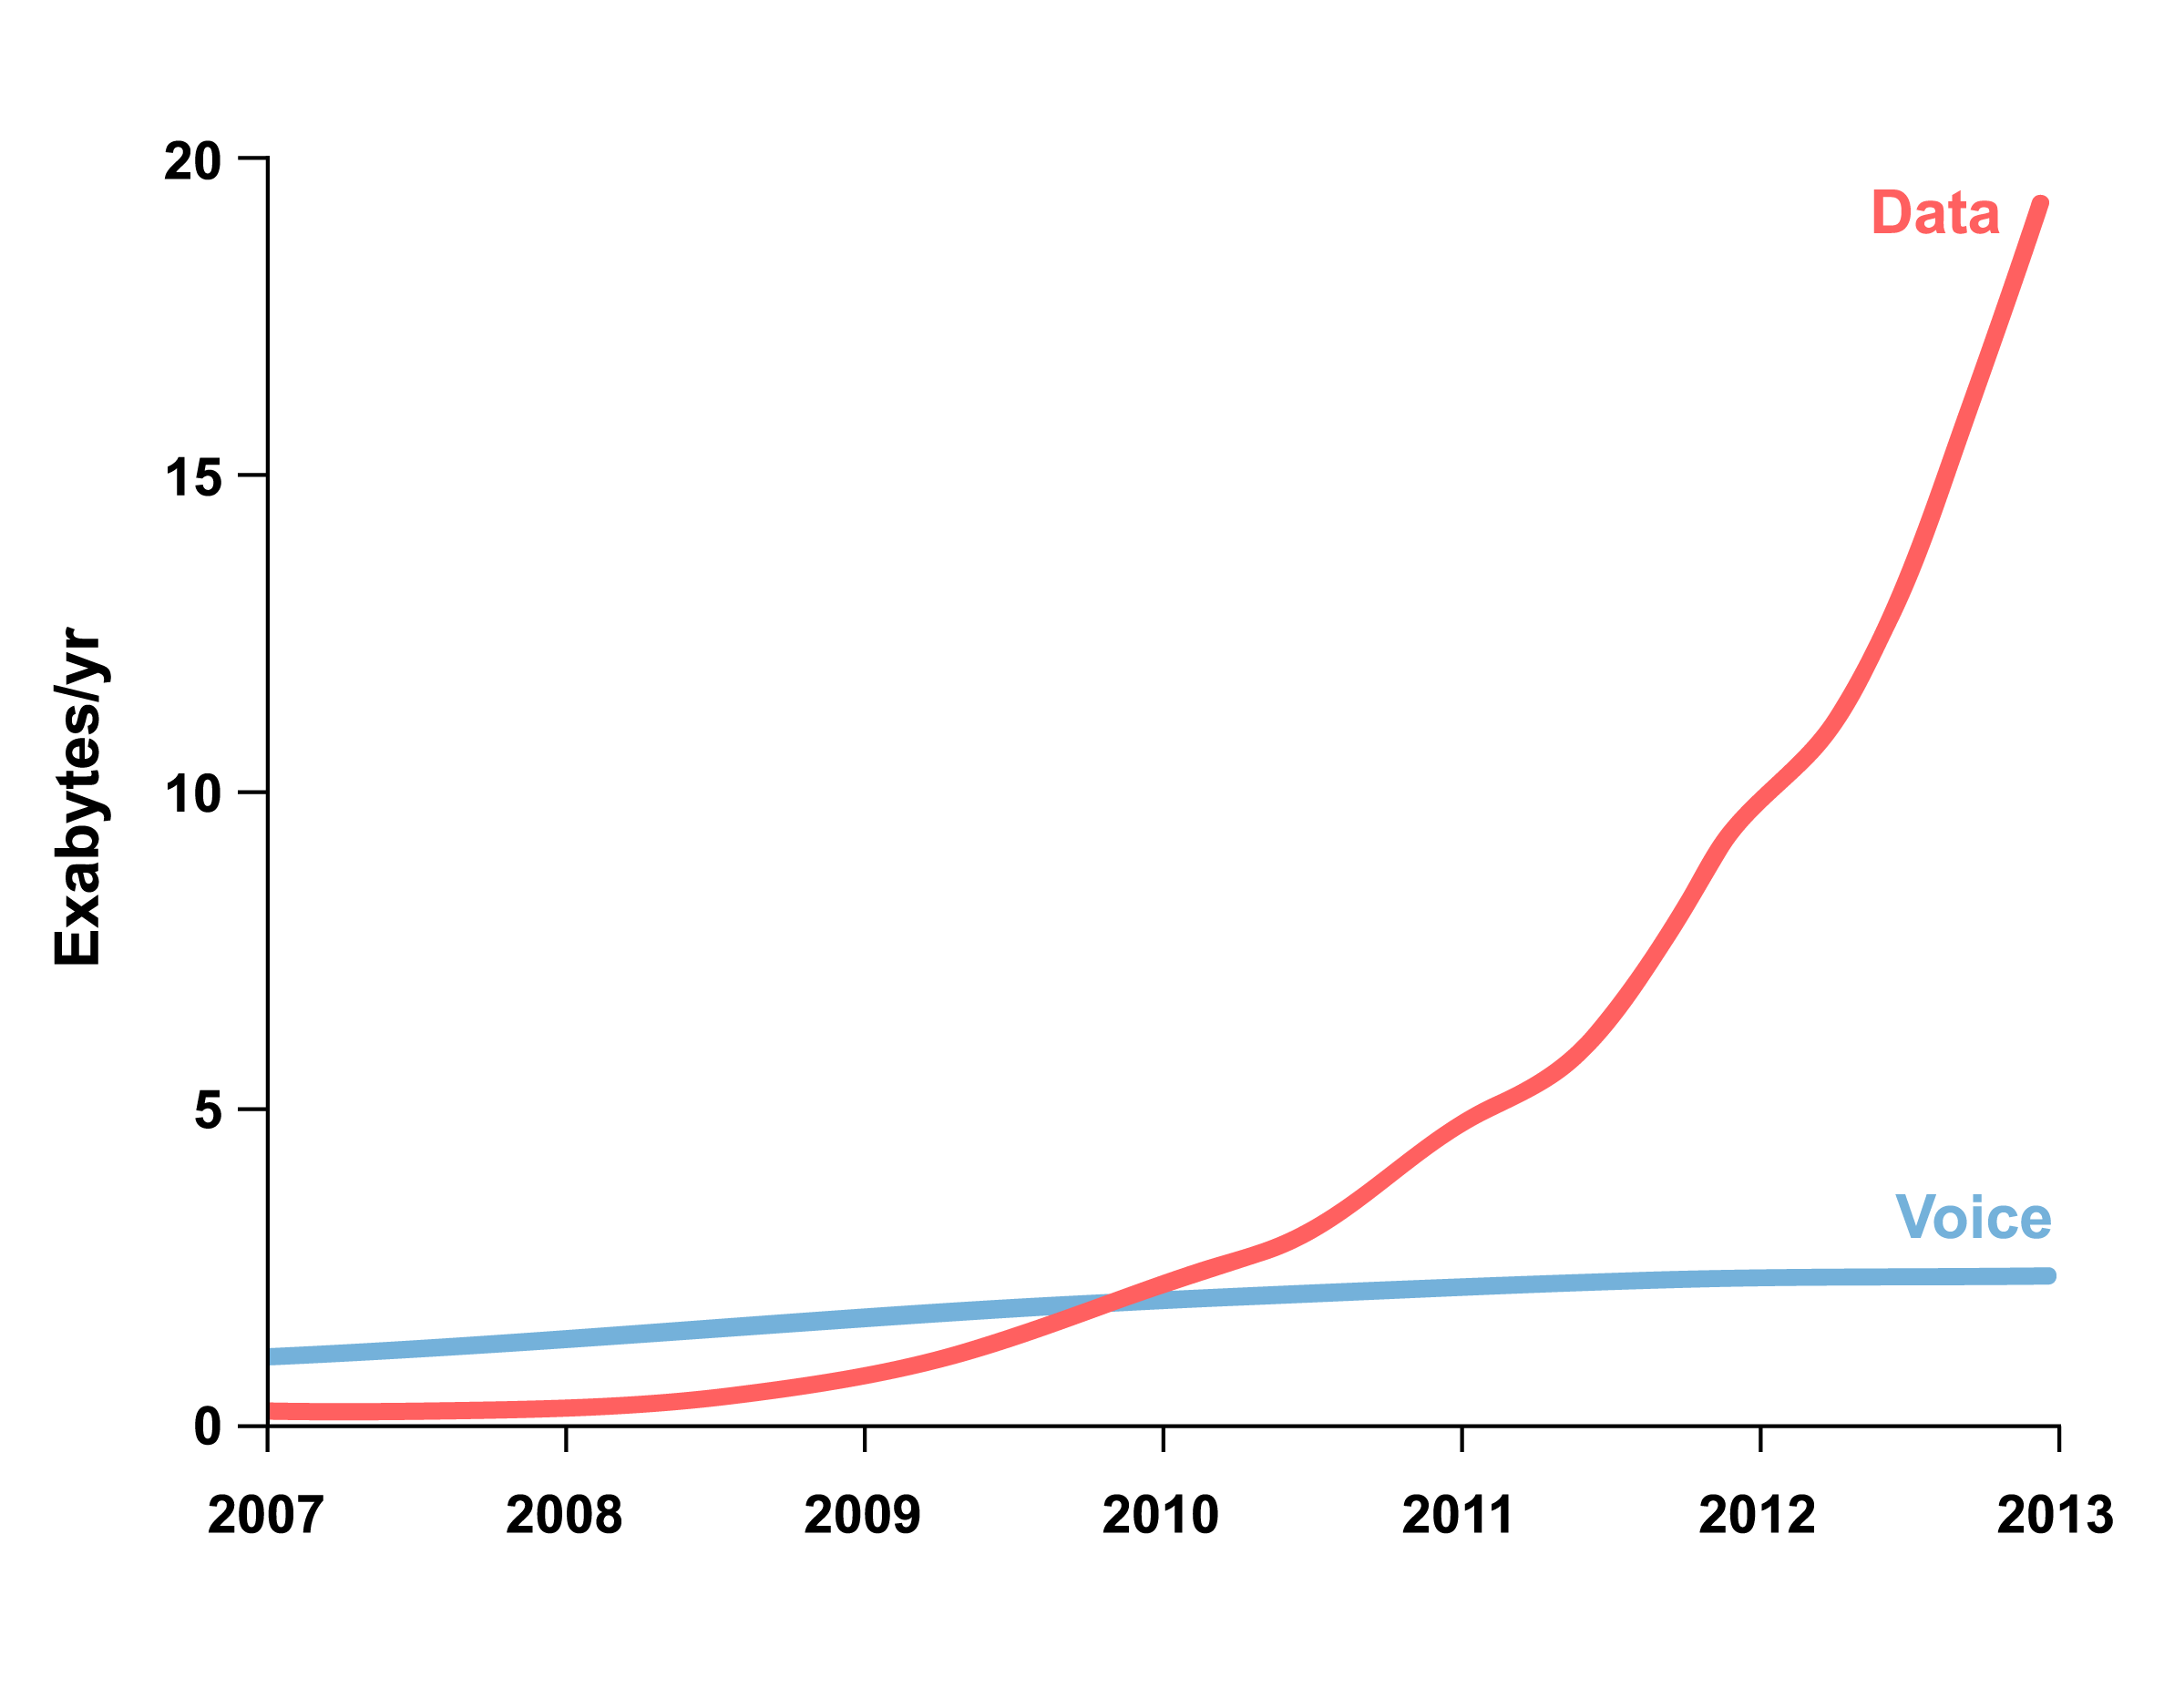
\includegraphics[scale=0.3]{imagens/consumo.png}
				    \caption{Consumo de dados e voz}
				    \label{fig:sample_figure}
				\end{figure}

	\end{frame}
	
		\begin{frame} {Motivação}
			
			\centering
			\normalsize	 
				Por causa disso, o número de servidores em Data Centers deve crescer exponencialmente para acompanhar a demanda, o que traz dificuldades em desenvolver redes eficientes e de baixo custo.
			\begin{figure}[ht]
	   
			   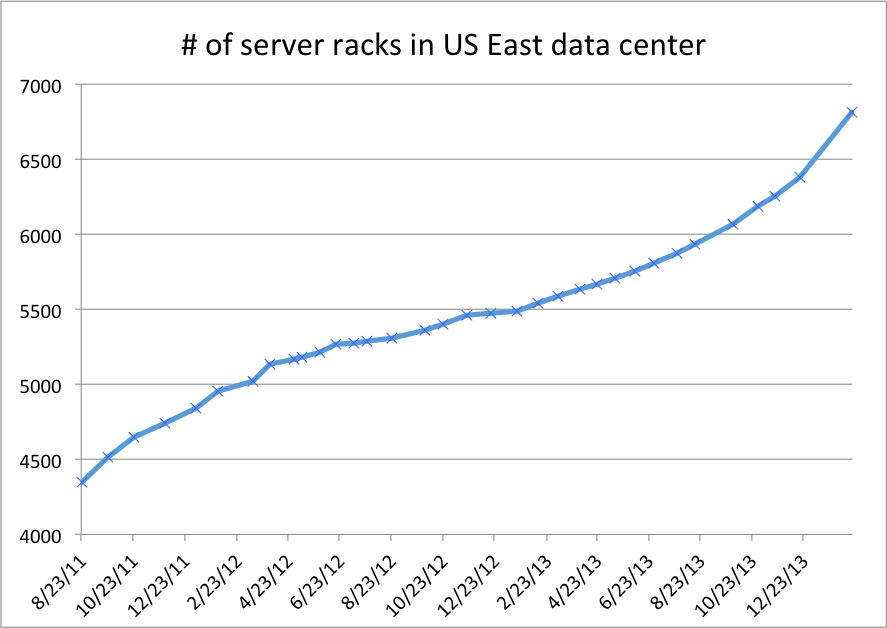
\includegraphics[scale=0.45]{imagens/servidores.png}
			    \caption{Número de servidores racks}
			    \label{fig:sample_figure}
			\end{figure}
		
		\end{frame}
		
		\begin{frame} {Motivação}
				
			\Large
			Disponibilidade de dados e segurança se tornaram aplicações críticas.
			
		\end{frame}
				
			
		\begin{frame} {Motivação}
				
			\Large
			Por outro lado, a criação de novas tecnologias faz com que o custo dos componentes seja cada vez menor.
			\begin{figure}[ht]    
						    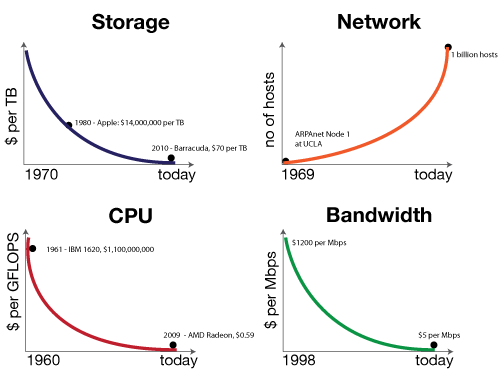
\includegraphics[scale=0.35]{imagens/custo.png}
						    \caption{Custo de tecnologias}
						    \label{fig:sample_figure}
						\end{figure}
		\end{frame}	
			
		
	
\section{Topologias}
	\subsection{Tradicionais}

	\begin{frame} {Topologias Tradicionais}
	\begin{itemize}
	 	\item
	 		Baseadas em Árvores:
			\begin{itemize}
			 	\item
			 		CLOS
			 	\item
					Basic Tree
			 	\item
					Fat-Tree
			 	\item
					VL2
			 \end{itemize}
	 	\item
	 		Recursivas:
			\begin{itemize}
			 	\item
			 		Dcell
			 	\item
					Bcube
			 	\item
					FiConn
			 	\item
					FlatNet
			 	\item
					SprintNet
			 \end{itemize}
	 \end{itemize}
	\end{frame}

	\begin{frame} {Topologias Tradicionais}
		Topologias baseadas em árvores
	\end{frame}

	\begin{frame} {Topologias Tradicionais}
		Topologias recursivas
	\end{frame}

	\begin{frame} {Topologias Recursivas: Dcell}
		Baseada em células interligadas entre servidores
		\begin{figure}[ht]    
			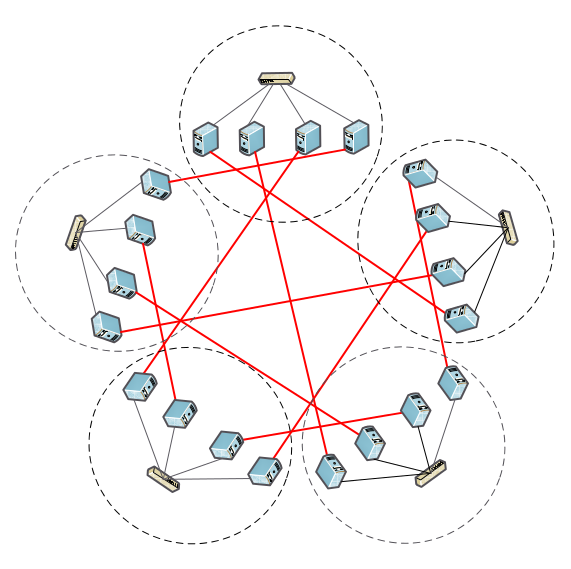
\includegraphics[scale=0.3]{imagens/dcell.png}
			\label{fig:sample_figure}
		\end{figure}
	\end{frame}

	\begin{frame} {Topologias Recursivas: Bcube}
		Baseada em células interligadas entre switches
		\begin{figure}[ht]    
			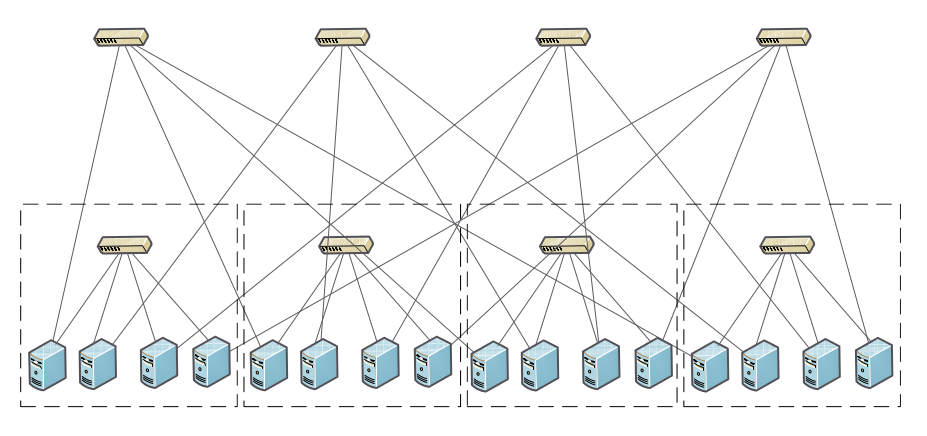
\includegraphics[scale=0.3]{imagens/bcube.png}
			\label{fig:sample_figure}
		\end{figure}
	\end{frame}

	\begin{frame} {Topologias Recursivas: FiConn}
		Semelhante à Dcell, mas o grau de cada célula é sempre 2
		\begin{figure}[ht]    
			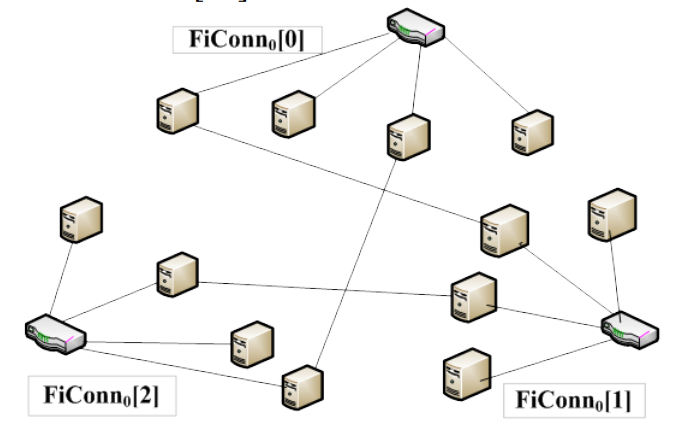
\includegraphics[scale=0.3]{imagens/ficonn.png}
			\label{fig:sample_figure}
		\end{figure}
	\end{frame}

	\begin{frame} {Topologias Recursivas: FlatNet}
		Semelhante ao BCube, porém é mais escalável
		\begin{figure}[ht]    
			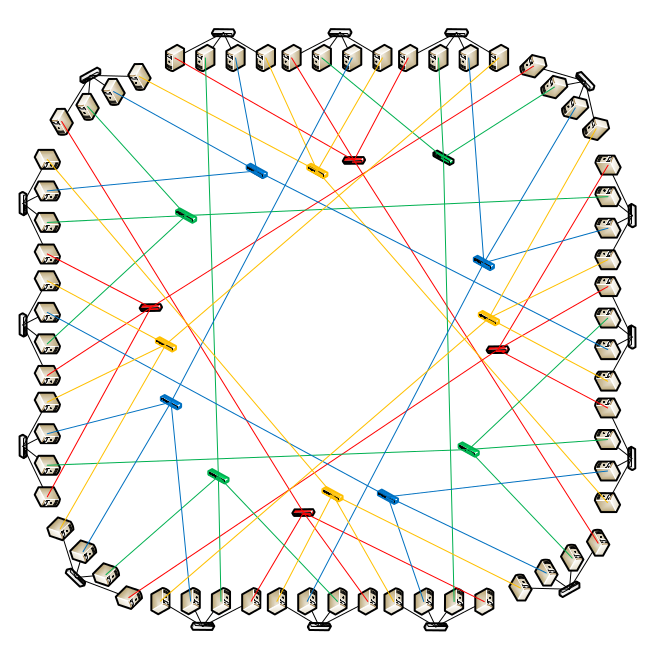
\includegraphics[scale=0.3]{imagens/flatnet.png}
			\label{fig:sample_figure}
		\end{figure}
	\end{frame}

	\begin{frame} {Topologias Recursivas: SprintNet}
		Semelhante à DCell, porém as células são compostas por 4 servidores e 2 switches de 6 portas
		\begin{figure}[ht]    
			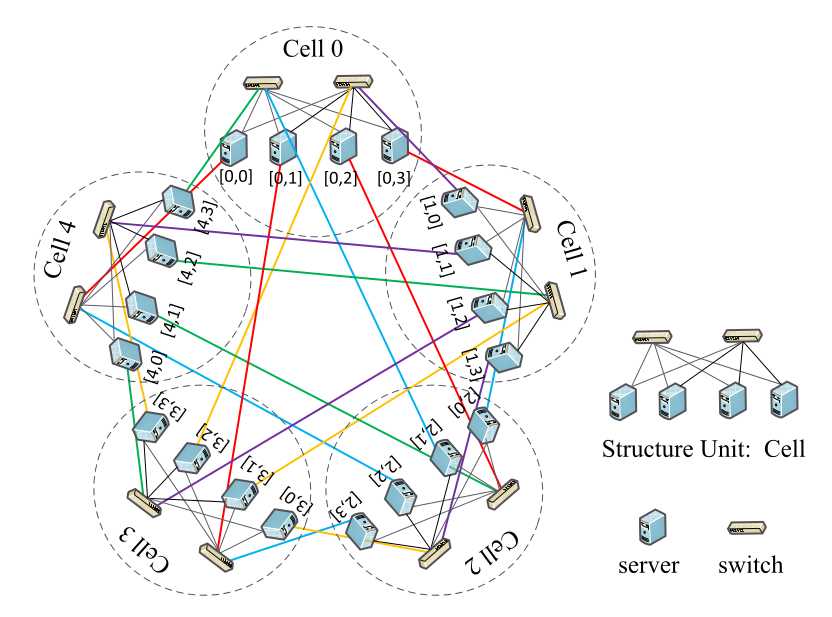
\includegraphics[scale=0.3]{imagens/springnet.png}
			\label{fig:sample_figure}
		\end{figure}
	\end{frame}

	\begin{frame} {Comparação}
		\begin{figure}[ht]   
			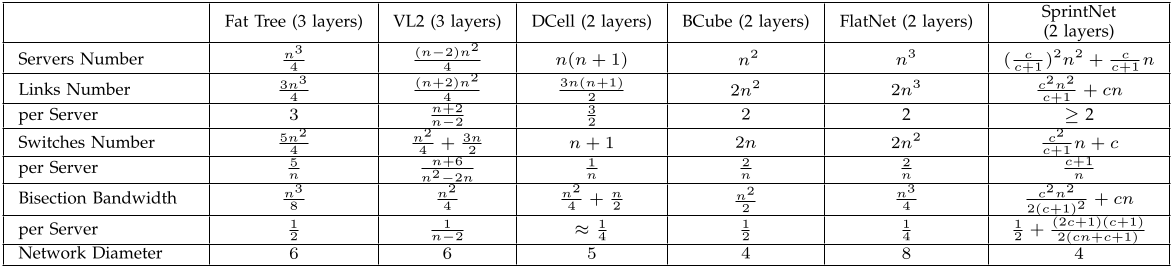
\includegraphics[scale=0.35]{imagens/tabela.png}
			\label{fig:sample_figure}
		\end{figure}
	\end{frame}

	\subsection{SDN}
		
	\begin{frame} {SDN em Datacenters}
		Com o avanço do SDN, a ideia mais básica é definir servidores virtualizados e criar uma rede virtualizada
		\begin{figure}[ht]   
			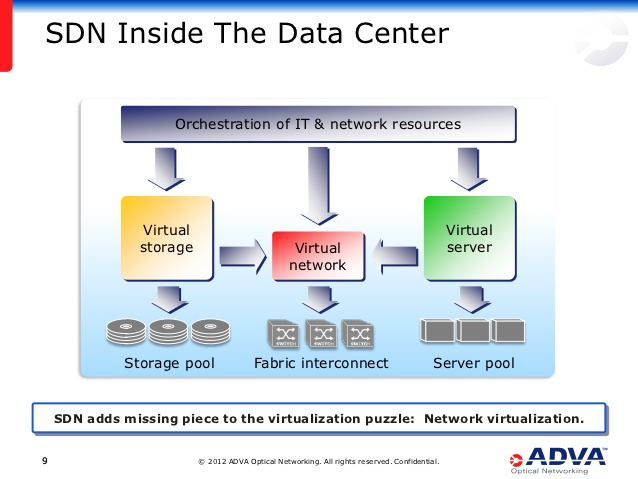
\includegraphics[scale=0.35]{imagens/inside-sdn.jpg}
			\label{fig:sample_figure}
		\end{figure}
	\end{frame}

	\begin{frame} {SDN em Datacenters}
		Esta técnica já é utilizada atualmente (PayPal por exemplo)
		\begin{figure}[ht]   
			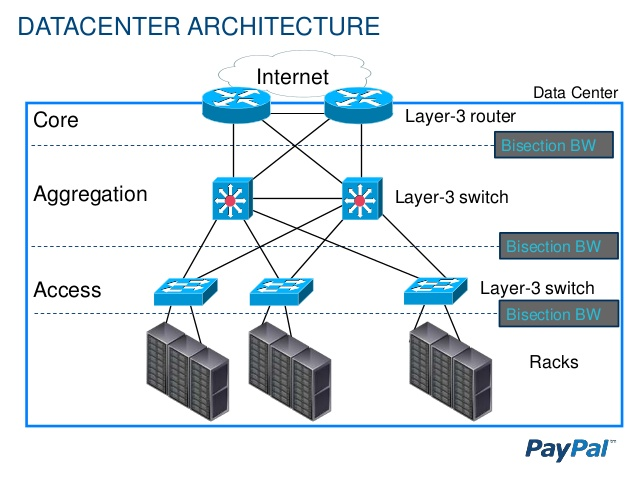
\includegraphics[scale=0.3]{imagens/sdn-1.jpg}
			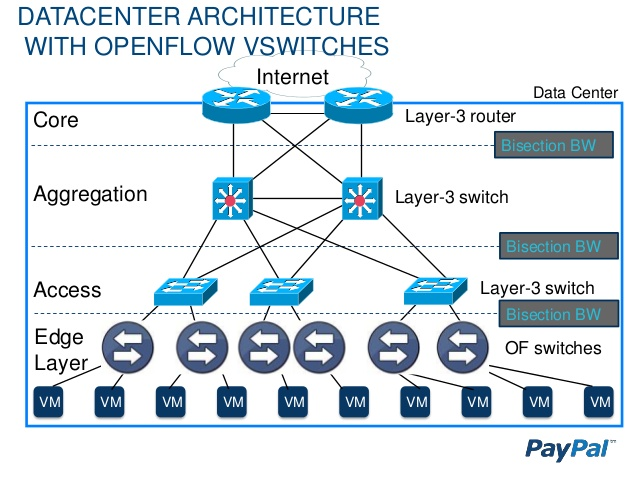
\includegraphics[scale=0.3]{imagens/sdn-2.jpg}
			\label{fig:sample_figure}
		\end{figure}
	\end{frame}

	\begin{frame} {SDN em Datacenters}
		\begin{figure}[ht]   
			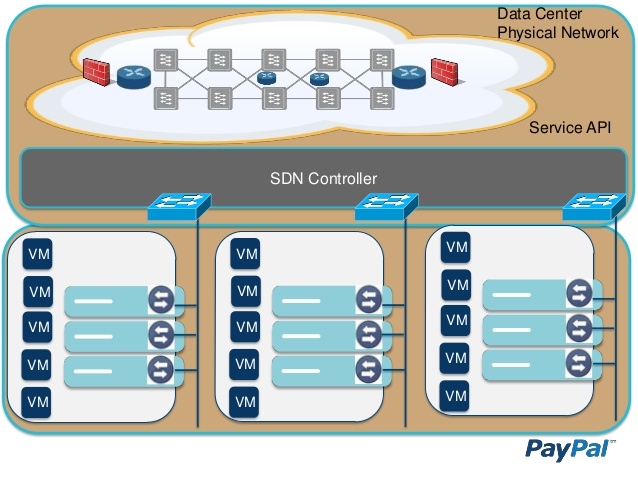
\includegraphics[scale=0.4]{imagens/sdn-3.jpg}
			\label{fig:sample_figure}
		\end{figure}
	\end{frame}

\section{Protocolos}{Protocolos}
	\subsection{Roteamento}
	\subsection{Comunicação}

	\begin{frame} {Protocolos de Comunicação}
	\begin{itemize}
	 	\item
	 		Deadline-Agnostic:
			\begin{itemize}
			 	\item
			 		$DCTCP$
			 	\item
					$MPTCP$
			 	\item
					$ICTCP$
			 \end{itemize}
	 	\item
	 		Deadline-Aware:
			\begin{itemize}
			 	\item
			 		$D^3$
			 	\item
					$D^2TCP$
			 	\item
					$DeTail$
			 	\item
					$PDQ$
			 \end{itemize}
	 \end{itemize}
	\end{frame}

	\begin{frame} {Protocolos de Comunicação}
		Protocolos Deadline-Agnostic
	\end{frame}

	\begin{frame} {Deadline-Aware: $D^3$}
		\begin{itemize}
		 	\item
		 		Recebe a informação do tamanho do fluxo e o deadline
		 	\item
				Algoritmo guloso para tentar cumprir o máximo de deadlines possíveis
		 	\item
				Roteadores tentam alocar uma taxa adequada para cada fluxo
		 	\item
				Emissor envia dados com a mínima taxa alocada no próximo RTT
		 	\item
				A fonte periodicamente requisita uma nova taxa baseada no deadline e o tamanho do fluxo restante
		 \end{itemize}
	\end{frame}

	\begin{frame} {Deadline-Aware: $D^3$}
		\begin{itemize}
		 	\item
		 		Switches precisam de modificações para lidar com as requisições
		 	\item
				Não é compatível com o TCP tradicional, por causa da alocação de largura banda baseado em prioridades sem a informação do deadline no header
		 	\item
				Alocação com algoritmo guloso pode alocar largura de banda para fluxos com deadlines distantes ao invés de deadlines próximos, o que pode causar maior perda de deadlines
		 	\item
				Requisições constantes de taxas tem um overhead
		 \end{itemize}
	\end{frame}

	\begin{frame} {Deadline-Aware: $D^2TCP$}
		\begin{itemize}
		 	\item
		 		Baseado no DCTCP, mas leva o deadline em consideração para redimensionar a janela de congestionamento
		 	\item
				Se a maioria dos deadlines são próximos, ainda pode ocorrer congestionamento
		 	\item
				Se a maioria dos deadlines são distantes, ocorrerá a sub-utilização da rede e baixa taxa de transferência
		 	\item
				Se todos os deadlines são próximos, estão competindo pela largura de banda e nenhum fluxo é adiado, todos os deadlines não serão cumpridos. Caso um fluxo seja adiado, todos os outros podem ser cumpridos.
		 	\item
				O problema é saber qual fluxo sacrificar para satisfazer o máximo de deadlines possíveis
		 \end{itemize}
	\end{frame}

	\begin{frame} {Deadline-Aware: $DeTail$}
		\begin{itemize}
		 	\item
		 		Fluxos são associados com prioridades e os switches usam filas de prioridades nas portas de saída e de entrada
		 	\item
				Cada camada da abstração da rede tem uma função
		 \end{itemize}

		\begin{figure}[ht]   
			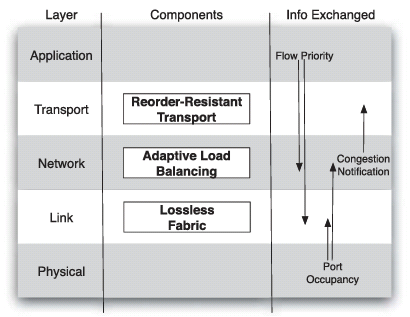
\includegraphics[scale=0.5]{imagens/detail.png}
			\label{fig:sample_figure}
		\end{figure}
	\end{frame}

	\begin{frame} {Deadline-Aware: $DeTail$}
		Enlace:
		\begin{itemize}
		 	\item
		 		Controle de fluxo “hop-by-hop” 
		 	\item
				Tenta amenizar o bloqueio de “head-of-line” (HOL)
		 	\item
				Recebe informações da camada de rede em relação ao balanco de carga adaptativo
		 	\item
				Recebe informações da camada de transporte sobre o estado do ECN
		 \end{itemize}
	\end{frame}

	\begin{frame} {Deadline-Aware: $DeTail$}
		Rede:
		\begin{itemize}
		 	\item
		 		Balanço de carga adaptativo baseado em pacotes de acordo com o nível de congestionamento
		 	\item
				Pode transmitir pacotes por caminhos que estão com pouca carga
		 \end{itemize}
	\end{frame}

	\begin{frame} {Deadline-Aware: $DeTail$}
		Rede:
		\begin{itemize}
		 	\item
		 		Usa o ECN para marcar fluxos de baixa prioridade quando os bytes transmitidos para o destino ultrapassam um certo limiar
		 	\item
				Previne congestionamento persistente
		 \end{itemize}
	\end{frame}

	\begin{frame} {Deadline-Aware: $DeTail$}
		Aplicação:
		\begin{itemize}
		 	\item
		 		Seleciona as prioridades de cada fluxo baseado na sensibilidade de latência
		 \end{itemize}
	\end{frame}

	\begin{frame} {Deadline-Aware: $PDQ$}
		\begin{itemize}
		 	\item
		 		Semelhante ao $D^3$, mas ao contrário do $D^3$, escalona taxas de acordo com a criticalidade dos fluxos ao invés da política “first-come first-serve”
		 	\item
		 		Duas políticas de alocação, implementadas de forma totalmente distribuída:
				\begin{itemize}
				 	\item
				 		EDF (Earliest Deadline First)
				 	\item
						SJF (Shortest Job First)
				 \end{itemize}
		\end{itemize}
	\end{frame}

\section{Tendências}
	\begin{frame} 
		Ponha aqui seu texto
	\end{frame}

\section{Conclusão}
	\begin{frame} 
		Ponha aqui seu texto
	\end{frame}
		
\section{Pergunta}
	\begin{frame} 
		Ponha aqui seu texto
	\end{frame}
	
\end{document}
